\input{../include/preamble}

\title[ID1019 Recursion]{Lists and recursion}


\author{Johan Montelius}
\institute{KTH}
\date{\semester}

\begin{document}

\begin{frame}
\titlepage
\end{frame}

\begin{frame}{first a recap}

\pause In functional programming, a program is a set of functions.

\vspace{20pt}\pause A function takes some arguments and {\em returns a result} \ldots it does not change the given arguments.

\vspace{20pt}\pause The returned value of a function is only depending on the given arguments.

\vspace{20pt}\pause Fundamentally different from {\em imperative programming}!


\end{frame}

\begin{frame}[fragile]{any difference?}

\begin{columns}
 \begin{column}{0.5\linewidth}
\begin{verbatim} 
def foo(x)  do
    y = bar(x)
    z = zot(x)
    {y, z}
end
\end{verbatim}
 \end{column}
 \pause  
  \begin{column}{0.5\linewidth}
\begin{verbatim} 
def grk(x) do
    z = zot(x)
    y = bar(x)
    {y, z}
end
\end{verbatim}
 \end{column}
\end{columns}

\vspace{40pt} 
\pause What is the difference between these two functions?

\end{frame}

\begin{frame}[fragile]{catch this}
\begin{verbatim}
def foo(x, y) do
    res = try do
              bar(x, y)
          rescue
              error ->
                  {:caught, error}
          end,
    {x, y, res}
end
\end{verbatim}
\end{frame}

\begin{frame}{today's topic}

\vspace{60pt}\hspace{80pt}Lists and recursion

\end{frame}

\begin{frame}{pattern matching}
\begin{itemize}
\pause \item  {\tt [h|t] = [:a,[:b,:c]]}  
\pause \item  {\tt [h1,h2|t] = [:a,:b,:c]} 
\pause \item  {\tt [h1,h2,t] = [:a,:b,:c]} 
\pause \item  {\tt [h1,h2,t] = [:a,:b,:c,:d]} 
\pause \item  {\tt [h1|[h2|t]] = [:a,:b,:c]}
\pause \item  {\tt [h|t] = [:a|:b]}
\end{itemize}
\end{frame}

\begin{frame}{list construction}
\begin{itemize}
\pause \item  {\tt h = :a; t = [:b]; [h|t]}
\pause \item  {\tt h = :a; t = [[:b]]; [h|t]}
\pause \item  {\tt h = [:a,:b]; t = [:c,:d]; [h|t]}
\pause \item  {\tt h = [:a,:b]; t = [:c,:d]; [h,t]}
\pause \item  {\tt h1 = [:a,:b]; h2 = [:c,:d]; t = [e,f]; [h1|[h2|t]]}
\pause \item  {\tt h1 = [:a,:b]; h2 = [:c,:d]; t = [e,f]; [h1,[h2|t]]}
\pause \item  {\tt h = [:a,:b]; t = :c; [h|t]}
\end{itemize}
\end{frame}


\begin{frame}{cons cells}

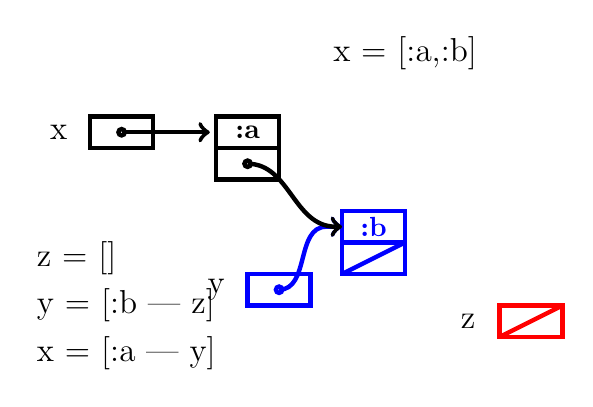
\begin{tikzpicture}[scale=0.4]

\node[anchor=west] at (0,3.5) {{\large z = []}};

\node at (14,1.5) {{\large z}};
\draw [ultra thick, red] (15,1) rectangle +(2,1);
\draw [ultra thick, red] (15,1) -- +(2,1);

\pause 
\node[anchor=west] at (0,2) {{\large y = [:b | z]}};
\pause 
\node at (6,2.5) {{\large y }};
\draw [ultra thick, blue] (7,2) rectangle +(2,1);
\pause 
\draw [ultra thick, blue] (10,4) rectangle +(2,1) node at +(1,0.5) {{\bf :b}};
\draw [ultra thick, blue] (10,3) rectangle +(2,1);
\draw [ultra thick, blue] (10,3) -- +(2,1);
\pause 
\draw [ultra thick, blue] (8, 2.5) circle [radius =0.1];
\draw [ultra thick, blue] (8,2.5)  to [out=0, in=180]  (9.5,4.5);
\draw [ultra thick, blue, ->] (9.5,4.5) -- (10,4.5); 

\pause 
\node[anchor=west] at (0,0.5) {{\large x = [:a | y]}};
\pause 
\node at (1,7.5) {{\large x }};
\draw [ultra thick, black] (2,7) rectangle +(2,1);
\pause 
\draw [ultra thick, black] (6,7) rectangle +(2,1) node at +(1,0.5) {{\bf :a}};
\draw [ultra thick, black] (6,6)  rectangle +(2,1);
\pause 

\draw [ultra thick, black] (7, 6.5) circle [radius =0.1];
\draw [ultra thick, black] (7,6.5)  to [out=0, in=180]  (9.8,4.5);
\draw [ultra thick, black, ->] (9.8, 4.5) -- (10,4.5);
\pause 
\draw [ultra thick, black] (3, 7.5) circle [radius =0.1];
\draw [ultra thick, black, ->] (3,7.5) -- (5.8, 7.5); 
\pause
\node at (12,10) {{\large x = [:a,:b] }};

\end{tikzpicture}

\end{frame}


\begin{frame}[fragile]{append}

\begin{verbatim}
def append([], y) do y end
def append([h|t], y) do
   z = append(t, y)
   [ h | z ]
end
\end{verbatim}

\pause
\begin{verbatim}
a = [1,2]; b = [3,4]; c = append(a, b)
\end{verbatim}

\pause

\begin{tikzpicture}[scale=0.4]
  
  \node at (0,8) {{\bf a } }; 
  \cell{0.5}{8}
  \pointer{0.5}{8}{2}{6}

  \cons{2}{6}{1}
  \cdrpointer{2}{6}{6}{4}

  \cons{6}{4}{2}
  \cdrnil{6}{4}

  \node at (8,8) {{\bf b }};
  \cell{8.5}{8}
  \pointer{8.5}{8}{12}{6}

  \cons{12}{6}{3}
  \cdrpointer{12}{6}{16}{4}

  \cons{16}{4}{4}
  \cdrnil{16}{4}

  \pause
  \cdrpointer{6}{0}{12}{6}

  \pause
  \cdrpointer{2}{0}{6}{0}
  \cons{6}{0}{2}

  \pause
  \pointer{0.5}{2}{2}{0}
  \cons{2}{0}{1}

  \pause
  \node at (0,2) {{\bf c }};
  \cell{0.5}{2}
  \pause


\end{tikzpicture}

\end{frame}



\begin{frame}[fragile]{append}

\begin{verbatim}
def append([], y) do y end
def append([h|t], y) do 
  [ h | append(t, y)] 
end
\end{verbatim}

\pause\vspace{20pt} What is the {\em asymptotic time complexity} of append/2.
\end{frame}


\begin{frame}{append}

\begin{tabular}{|l|c|}
\hline
length of X & run-time in ms\\
\hline
  4000  &     50 \\
  8000  &     78 \\
 10000  &     75 \\
 12000  &     99 \\
 14000  &    102 \\
 16000  &    110 \\
 18000  &    122 \\
 20000  &    150 \\
\hline
\end{tabular}

\pause \vspace{20pt}How long time does it take to append a list of 40.000 elements?

\end{frame}

\begin{frame}{warning}

\pause The infix operator '++' is append! 

\pause\vspace{20pt} {\tt x ++ y} is not a constant time operation!

\pause\vspace{20pt} Is {\tt [x|y]} a constant time operation?

\end{frame}

\begin{frame}[fragile]{union of multisets}

A {\em multiset} (or bag) is a set possibly with duplicated elements.

\pause \vspace{20pt} Define a function that returns the union of two multisets.
\pause

\begin{columns}
  \begin{column}{0.5\textwidth}
\begin{verbatim}
def union([], y) do y end
def union([h|t], y) do
   z = union(t,y)
   [h|z]
end
\end{verbatim}
  \end{column}
\pause
  \begin{column}{0.5\textwidth}
\begin{verbatim}
def tailr([], y) do y end
def tailr([h|t], y) do 
  z = [h|y]
  tailr(t,z)
end
\end{verbatim}
  \end{column}
\end{columns}

\pause\vspace{20pt} Is there a difference?

\end{frame}

\begin{frame}[fragile]{evaluation union vs tailr}

\begin{columns}
  \begin{column}{0.5\textwidth}
\pause{\tt union([:a,:b], [:c])})\\
\pause\hspace{20pt}{\tt z = union([:b], [:c])})\\
\pause\hspace{40pt}{\tt z' = union([],[:c])})\\
\pause\hspace{60pt}{\tt [:c]}\\
\pause\hspace{40pt}{\tt [:b|z']}\\
\pause\hspace{20pt}{\tt [:a|z]}\\
\pause$[:a,:b,:c]$
\end{column}
\begin{column}{0.5\textwidth}
\pause{\tt tailr([:a,:b], [:c])})\\
\pause\hspace{20pt}{\tt tailr([:b], [:a, :c])})\\
\pause\hspace{40pt}{\tt tailr([],[:b,:a,:c])})\\
\pause\hspace{60pt}{\tt [:b,:a:,:c]}\\
\pause\hspace{40pt}{\tt [:b,:a:,:c]}\\
\pause\hspace{20pt}{\tt [:b,:a:,:c]}\\
\pause$[:b,:a,:c]$
\end{column}
\end{columns}

\end{frame}


\begin{frame}{tail recursion optimization}

When the last expression in a sequence is a function call, the stack
frame of the caller can be reused.

\pause\vspace{20pt}We call these functions {\em tail recursive}.

\pause\vspace{20pt}Possibly more efficient code.

\pause\vspace{20pt}Probably more complicated.

\pause\vspace{20pt}Very important when we will define processes!

\end{frame}

\begin{frame}[fragile]{tail recursive?}

\begin{verbatim}
def sum([]) do 0 end
def sum([n|t]) do 
  n + sum(t) 
end
\end{verbatim}

\pause
\begin{verbatim}
def sum([]) do 0 end
def sum([n|t]) do 
  s = sum(t)
  n + s
end
\end{verbatim}

\end{frame}

\begin{frame}[fragile]{accumulators}

\begin{verbatim}
def odd([]) do  ... end
def odd([h|t]) do
   if rem(h,2) == 1 do
       ... 
   else 
       ...
   end
end
\end{verbatim}
\pause

\begin{verbatim}
def odd_n_even(l) do
   odd = odd(l),
   even = even(l),
   {odd, even}
end
\end{verbatim}
\end{frame}

\begin{frame}[fragile]{accumulators}

\begin{verbatim}
do odd_n_even([]) do
   {..., ...}
end
\end{verbatim}
\pause
\begin{verbatim}
def odd_n_even([h|t]) do
  {odd, even} = odd_n_even(t)
  if rem(h,2) == 1 do
    ...
  else 
     ...
  end
end
\end{verbatim}

\vspace{40pt}
{\em We're building a tuple that is not needed, its only purpose is to return the two lists.}

\end{frame}


\begin{frame}[fragile]{accumulators}

\pause
\begin{verbatim}
def odd_n_even(l) do 
   odd_n_even(l, [], [])
end
\end{verbatim}

\pause
\begin{verbatim}
def odd_n_even([], odd, even) do
   ...
end
\end{verbatim}
\pause
\begin{verbatim}
odd_n_even([h|t], odd, even) do
   if rem(h,2) == 1  do 
     odd_n_even(t, ..., ...)
   else
     odd_n_even(t, ..., ...) 
   end
end
\end{verbatim}

\end{frame}

\begin{frame}[fragile]{tail recursive?}

\begin{verbatim}
def sum(l) -> sum(l, ...) end

def sum([], s) do ... end
def sum([n|t], s) do sum(t, ...) end
\end{verbatim}

\end{frame}



\begin{frame}[fragile]{n-reverse}

  A function that reverses a list:

  \hspace{40pt}\verb+rev([1,2,3,4]) -> [4,3,2,1]+
  
\pause

\begin{columns}
  \begin{column}{0.5\linewidth}
\begin{verbatim}
def rev([]) do  [] end
def rev([h|t]) do
   rev(t) ++ [h]
end
\end{verbatim}
  \end{column}
\pause
  \begin{column}{0.5\linewidth}
\begin{verbatim}
def rev(l) do rev(l, []) end

def rev([], res) do res end
def rev([h|t], res) do 
  rev(t, [h|res]) 
end
\end{verbatim}
  \end{column}
  \end{columns}  
\end{frame}


\begin{frame}[fragile]{n-flatten}

  A function that flattens a list of list:

  \hspace{40pt}\verb+flatten([[1,2],[3,4]]) -> [1,2,3,4]+  
\pause

\begin{columns}
  \begin{column}{0.5\linewidth}
\begin{verbatim}
def flat([]) do  [] end
def flat([h|t]) do
   h ++ flat(t)
end
\end{verbatim}
  \end{column}
\pause
  \begin{column}{0.5\linewidth}
\begin{verbatim}
def flat(l) do flat(l, []) end

def flat([], res) do res end
def flat([h|t], res) do 
  flat(t, res ++ h) 
end
\end{verbatim}
  \end{column}
  \end{columns}  
\end{frame}


\begin{frame}{Summary}

\begin{itemize}
 \pause\item Pattern matching of lists - learn it by heart
 \pause\item cons - is a constant time operation
 \pause\item append - is a $O(n)$ function
 \pause\item tail recursion - a technique to master 
 \pause\item think about complexity
\end{itemize}

\end{frame}


\end{document}


